\section{Setting of the learning problem}

\subsection{Learning problem definition}

Can be defined as 3 components:

\begin{itemize}
	\item
	      A \uline{generator} \(G\) of random data \(x\) from a
	      probability distribution \(P(x)\)which is fixed and unknown to us.
	\item
	      A \uline{supervisor} \(S\) which returns an output value ${y \in Y}$
	      for each everyinput \(x \in X\) according to a conditional
	      probability distribution \(P(y | x)\), also fixed and unknown
	      to us.
	\item
	      A \uline{learning machine (algorithm)} \(L\) which is capable of
	      implementing(computing) any of a set of functions (models).
	      \(f_\theta\) where \(\theta\) is a set of parameters belonging to the
	      parameter space \(\theta\).
\end{itemize}

The selection of the best possible model according to \(L\) is done
based on a learning data sample
\(D = {(x_1, y_1), (x_2, y_2), ..., (x_n, y_n)}\) (where \(x_1\) are
vectors)

\subsection{Why is the relation between X and Y stochastic?}

In most of the cases, randomness is ignorance of the true effects.

\begin{enumerate}
	\item
	      Ignorance of the functional dependence on a not measured variable
	      \(z\).
	\item
	      Technical invisibility
\end{enumerate}

\subsection{Loss function}

\emph{loss fn} is a function
\(L: Y \times Y \longrightarrow \mathds{R}+\) such that:

\begin{enumerate}
	\item
	      \(L(y, y') = L(y', y)\) (symmetry)
	\item
	      \(L(y, y') = 0  \Longleftarrow y = y'\)
\end{enumerate}

Examples of loss functions:

\begin{itemize}
	\item
	      \(L(y, y') := 1\) if \(y \neq y'\) (0-1 loss) (zero-one) \(L_{01}\)
	\item
	      \(L(y, y') := (y - y')^2\) (squared error)
\end{itemize}

\subsection{Hypothesis space}

\[
	\mathcal{F} = \{f_\theta: \mathcal{X} \rightarrow \mathcal{Y} \mid \theta \in \varTheta \subseteq \mathds{R} \}
\]

\subsection{classifier}

Is a function \(f: X \longrightarrow Y\)

\(Y\) is a set of different symbols.

\subsection{Risk}

The risk of a function is its \textbf{expected loss}. Also known as true
error or generalization error.

\[\mathds{R}[f] := \mathds{E}_{(x, y) ~ p} [ L(f(x), y) ]
\]

A function that takes a function as an argument is called a functional.
Risk is a functional.

\subsection{Empirical error}

The average error or loss function evaluated on a specific data sample
\(D\).

\[\hat{R}_{D^n}[f] = \frac{1}{n} \sum_{i=1}^n L(f(x_i), y_i)
\]

This is also a functional.

\subsection{Training error}

The training error is the \textbf{empirical error} obtained in the data
sample used fortraining.

\subsection{Model error proposition}

*Proposition:* for a fixed model \(f_θ\) the expected value of the
empirical error based on a data sampleis equal to the true error.

\[\mathds{E}_{D^{ijd}p^n}[\hat{R}_{D^n}[f]] = R[f]
\]

\begin{proof}

	\begin{itemize}
		\item
		      TODO
	\end{itemize}
\end{proof}

\subsection{discriminative vs generative classifiers}

\subsubsection{Generative}

Example: Gaussian Naive Bayes

\subsubsection{Discriminative}

Example: Logistic regression

\subsection{Risk minimizers}

\subsubsection{Proposition}

The function minimizing the risk on the zero-one loss is the Bayes
classifier.Which is the one that given x, assigns the class with the
highest posterior probability.

\(f^* = argmax_{P(w | x)}\)

And the risk of \(f_{01}^*\) is the Bayes risk.

The upper bound of the Bayes risk is 0.5

\subsection{Regression under the square error / loss function}

\subsubsection{Standard setting of the regression problem}

\paragraph{Proposition}

We cannot compute this in practice since we do not know the distribution
of the data.

\paragraph{Proposition}

The bias / variance decomposition of the mean squared error.

\[MSE[f] = Bias(f)^2 + Var(f)
\]

There is a trade-off between bias and variance, known as the
bias-variance dilemma.

\paragraph{Remainder}

Given a dataset \(D = {x^i, y^i}\) of size \(n\)\((x^i, y^i)~p\) We
choose a loss function \(L\) and a hypothesis space \(F\).

\[F := { x \rightarrow f_\theta(x), \theta \in \Theta }
\]

\subparagraph{Observations}

The set of functions we chose matters a lot. In some sense \(F\) should
be large to minimize the chancesthat the choosen function is not in
\(F\).

\begin{itemize}
	\item
	      Chosing a Machine Learning Algorithm of \(F\) given a particular
	      \(D_n\)obviousley depends on this
	      \(D_n\).\(D_n! \rightsquigarrow f_\theta = f_n\)
	\item
	      The best possible solution \(f^*_{sq.}\) may not belong to \(F\).
\end{itemize}

In case \(f^*_{sq.} \notin F\) then we should
find:\(\hat{f}_{sq.} = argmin_{|| f - f^*_{sq.} ||}\)We could use
different norm functions.

The expression being integrated is:

\[\left( f_m(x) - f^*_{sq.}(x) \right)^2
\]

Expected value of the model for all possible datasets in \(D_n\):

\(Bias^2(f_n(x))\) : how the average prediction over all possible
\(D_n\) at point \(x\)differs from the best possible predicition.

\[Bias^2(f) = \int_{\mathds{R}^d} \left( \overline{f_n}(x) - f_{sq.}^*(x) \right)^2 p(x) dx
	Var(f) = \int_{\mathds{R}^d} \mathds{E}_{D_n} \left[ \left( f_n(x) - \overline{f_n}(x) \right)^2 \right] p(x) dx
\]

\[MSE[f] = Bias(f)^2 + Var(f) + \sigma^2
\]

where \(\sigma^2\) is the variance of the noise.

Since \(\sigma\) cannot be reduced, it is called irreducible error.The
rest is called reducible error.

Getting better data we reduce the irreducible error. (ignorance)

\section{Consistency}

We depart from a specific data sample \(D_n\)The training error of a
model \(f\) is
\(\hat{R}_n^{[f]} := \frac{1}{n} \sum_{i=1}^n L(f(x^i), y^i)\)

So when we learn a specific model \(f_n\) from \(D_n\) its
\textbf{training error} is \(\hat{R}_n(f_n)\)The true error of \(f_n\)
is \(R(f_n)\)

The \uline{Empirical Risk Minimization} (ERM) prescribes to minimize the
training error.

\begin{description}
	\item[Consistency]
		The ERM is said to be \uline{consistent} if:

		\begin{itemize}
			\item
			      \(\hat{R}_n(f_n) \rightarrow {infimum}_{f \in F} R(f)\) as
			      \(n \rightarrow \infty\)
			\item
			      \(R(f_n) = \rightarrow {infimum}_{f \in F} R(f)\) as
			      \(n \rightarrow \infty\)
		\end{itemize}

		These convergences are in probability.
\end{description}

Graphically:

% \begin{verbatim}
% |******
% |      *****   R(f_n)
% |           ***************
% |                          ********
% |----------------------------------  converges -> infimum_{f \in F} R(f)
% |                          ********
% |           ***************
% |      *****   \hat{R}_n(f_n)
% |******                           n
% |---------------------------------->
% \end{verbatim}

\begin{figure}[H]
	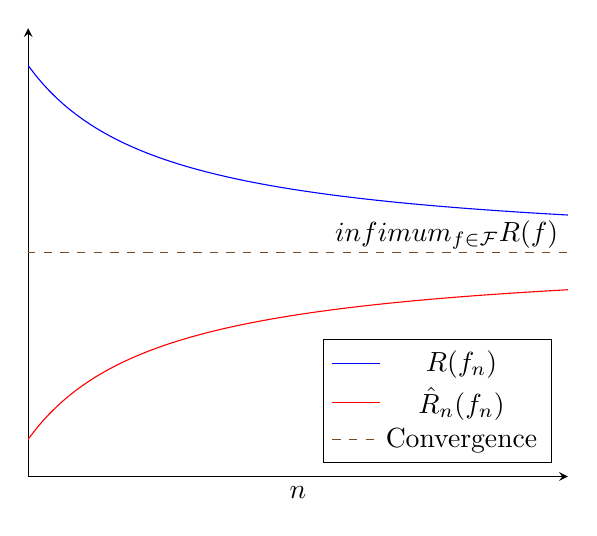
\begin{tikzpicture}
		\begin{axis}[
				domain=0.1:1.1,
				xmin=0.2, xmax=1,
				ymin=-6, ymax=6,
				samples=100,
				axis y line=center,
				axis x line=bottom,
				xlabel = {$n$},
				legend pos=south east,
				% area style,
				ticks=none,
			]
			\addlegendentry{\(R(f_n)\)};
			\addlegendentry{\(\hat{R}_n(f_n)\)};
			\addlegendentry{Convergence};
			\addplot+[mark=none] {1/x};
			\addplot+[mark=none] {-1/x};
			\addplot+[mark=none,dashed] {0};
			\node at (axis cs:1,1.1) [anchor=north east] {\(infimum_{f \in \mathcal{F}} R(f)\)};
		\end{axis}

	\end{tikzpicture}
	\caption{Convergence of the training error and the true error}
\end{figure}

\begin{description}
	\item[Theorem (Vapnik-Chervonenkis) P1]
		A necessary and sufficient condition for consistency is that the
		hypothesis space \(F\) is compact.

		\[\forall \varepsilon >
		\]
\end{description}
